
\begin{tabular}[t]{>{}cccccc}
\toprule
\multicolumn{2}{c}{  } & \multicolumn{4}{c}{Sample Size} \\
\cmidrule(l{3pt}r{3pt}){3-6}
  & Distribution & 50 & 100 & 400 & 1000\\
\midrule

\includegraphics[width=0.67in, height=0.17in]{distribution_table_a.pdf} & Laplace & 83.6\% & 79.6\% & 80\% & 80\%\\

\includegraphics[width=0.67in, height=0.17in]{distribution_table_b.pdf} & T & 83.3\% & 78.9\% & 79.8\% & 80\%\\

\includegraphics[width=0.67in, height=0.17in]{distribution_table_c.pdf} & Normal & 81.6\% & 76.2\% & 79.7\% & 79.9\%\\
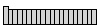
\includegraphics[width=0.67in, height=0.17in]{distribution_table_d.pdf} & Uniform & 79.8\% & 73.2\% & 79.5\% & 79.9\%\\

\includegraphics[width=0.67in, height=0.17in]{distribution_table_e.pdf} & Beta & 78.1\% & 68.8\% & 79.3\% & 79.9\%\\

\includegraphics[width=0.67in, height=0.17in]{distribution_table_f.pdf} & Sparse 3 & 85\% & 82.6\% & 81.9\% & 81.9\%\\

\includegraphics[width=0.67in, height=0.17in]{distribution_table_g.pdf} & Sparse 2 & 87.5\% & 85.6\% & 84.5\% & 84.4\%\\

\includegraphics[width=0.67in, height=0.17in]{distribution_table_h.pdf} & Sparse 1 & 92.6\% & 91\% & 90.3\% & 90.4\%\\
\bottomrule
\end{tabular}
